\begingroup
\newcolumntype{L}[1]{>{\hsize=#1\hsize\raggedright\arraybackslash}X}

\section{Hình ảnh minh chứng bắt buộc}
\label{sec:evidence}
Phần này lưu trữ ảnh chụp trạng thái trước và sau khi cấu hình bộ định tuyến/điểm truy cập, thông
tin kết nối của Laptop, Desktop, Smartphone và minh chứng kiểm tra Ad-hoc tối
thiểu hai nút ping được nhau. Ảnh minh chứng cấu hình bộ định tuyến/điểm truy cập được trích trực
tiếp từ video minh chứng (Mục~\ref{sec:video}); ảnh minh chứng Ad-hoc lấy từ bộ
ảnh chụp màn hình của nhóm. Trước khi đưa ảnh vào báo cáo phải che mật khẩu, địa
chỉ quản trị nhạy cảm và dữ liệu cá nhân; các ảnh dưới đây đã che phần khóa Wi-Fi
và mật khẩu quản trị.

\subsection{Minh chứng cấu hình bộ định tuyến/điểm truy cập}
\label{subsec:evidence-infra}

Bộ định tuyến được cấu hình lại từ trạng thái mặc định của OpenWrt: trang quản trị
truy cập qua \texttt{192.168.1.1}, đặt mật khẩu cho tài khoản \texttt{root}, đổi
tên thiết bị thành \texttt{N09-Router} và đặt múi giờ Việt Nam. Hình~\ref{fig:luci-wifi24}
và Hình~\ref{fig:luci-wifi5} là cấu hình hai bộ phát;
Hình~\ref{fig:luci-overview} là trang Wireless sau khi áp dụng, cho thấy cả hai
bộ phát đều đang hoạt động và mỗi bộ phát có một \ac{bssid} riêng -- đúng với
phân tích ở Mục~\ref{sec:arch}.

\begin{figure}[htbp]
  \centering
  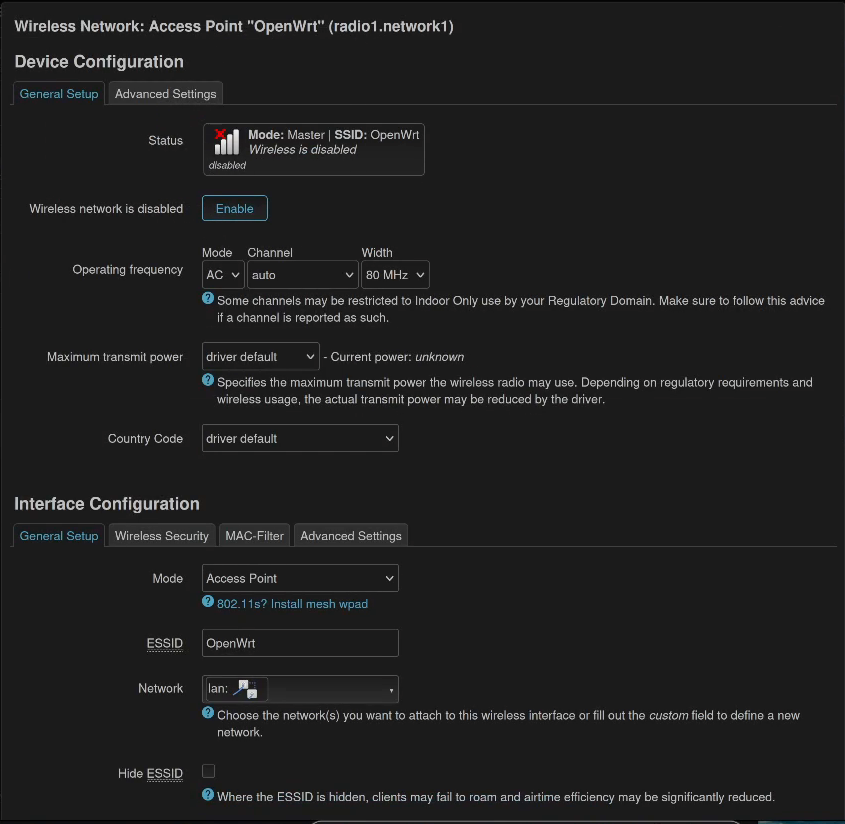
\includegraphics[width=\linewidth]{figures/N09_luci_wifi_24ghz.png}
  \caption[Cấu hình bộ phát 2,4 GHz trên LuCI]{Cấu hình bộ phát 2,4~GHz trên LuCI: mã quốc gia VN, Mode N, kênh~6,
  độ rộng 20~MHz, \ac{ssid} \texttt{25CLC04-N09}, bảo mật WPA2-PSK với mã hóa
  CCMP.}
  \label{fig:luci-wifi24}
\end{figure}

\begin{figure}[htbp]
  \centering
  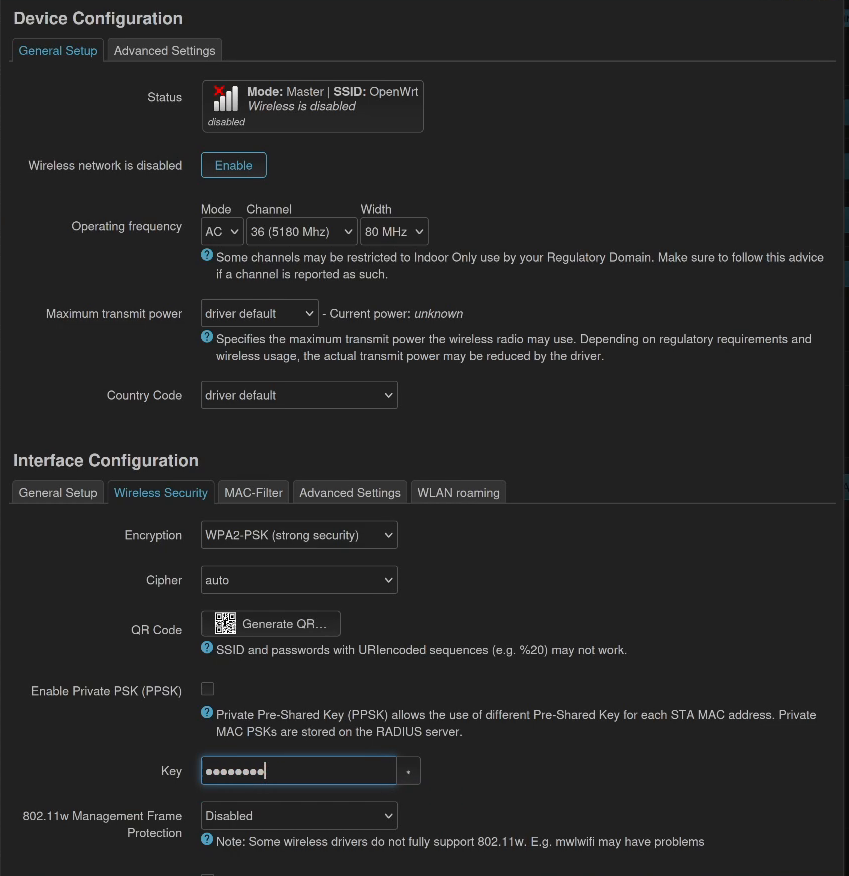
\includegraphics[width=\linewidth]{figures/N09_luci_wifi_5ghz.png}
  \caption[Cấu hình bộ phát 5 GHz trên LuCI]{Cấu hình bộ phát 5~GHz trên LuCI: chế độ AC, kênh~36, độ rộng 80~MHz,
  \ac{ssid} \texttt{25CLC04-N09-5G}.}
  \label{fig:luci-wifi5}
\end{figure}

\begin{figure}[htbp]
  \centering
  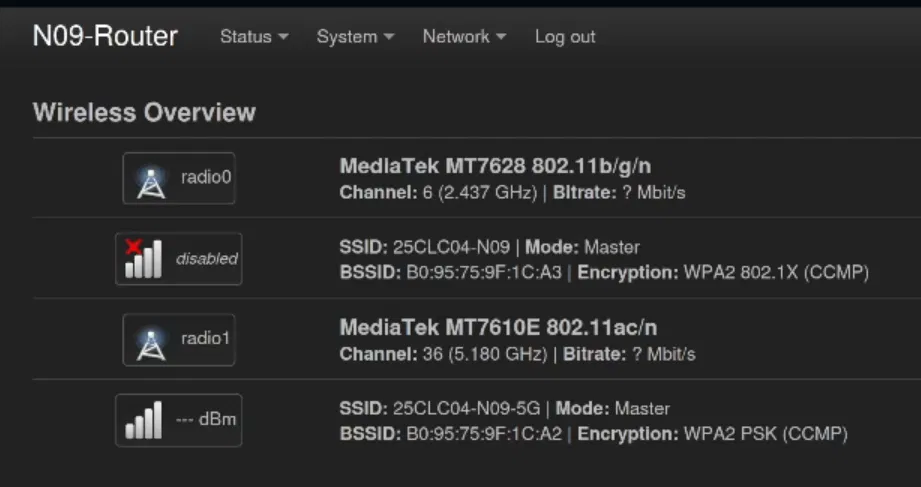
\includegraphics[width=\linewidth]{figures/N09_luci_wireless_overview.png}
  \caption[Hai bộ phát đang hoạt động trên trang Wireless]{Trang Wireless sau khi \emph{Save \& Apply}: hai bộ phát (MediaTek
  MT7628 2,4~GHz và MT7610E 5~GHz) đều đang phát, mỗi bộ phát có một
  \ac{bssid} riêng.}
  \label{fig:luci-overview}
\end{figure}

Cấu hình cấp địa chỉ được kiểm chứng bằng danh sách thuê DHCP trên router
(Hình~\ref{fig:luci-leases}) và bằng việc đặt địa chỉ IP tĩnh theo địa chỉ MAC
cho máy bàn (Hình~\ref{fig:luci-static}). Bảng~\ref{tab:dhcp-leases} tổng hợp
danh sách thiết bị đọc được từ hai nguồn này và từ sơ đồ
Hình~\ref{fig:sodo-n09}.

\begin{figure}[htbp]
  \centering
  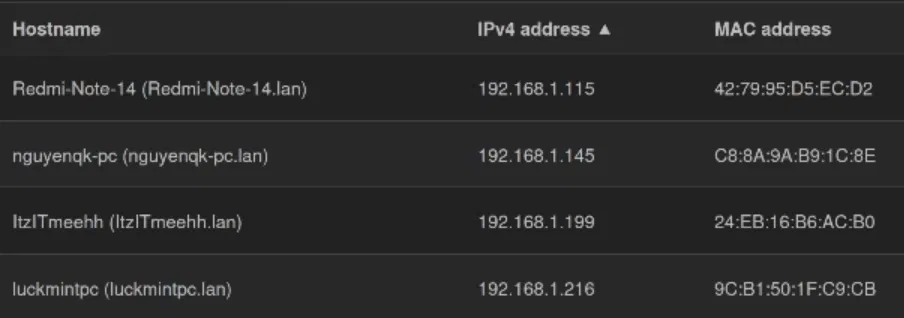
\includegraphics[width=\linewidth]{figures/N09_luci_dhcp_leases.png}
  \caption[Danh sách thuê DHCP thực tế trên N09-Router]{Danh sách thuê DHCP thực tế trên N09-Router: bốn thiết bị của nhóm đã
  nhận địa chỉ trong dải \texttt{192.168.1.0/24}.}
  \label{fig:luci-leases}
\end{figure}

\begin{figure}[htbp]
  \centering
  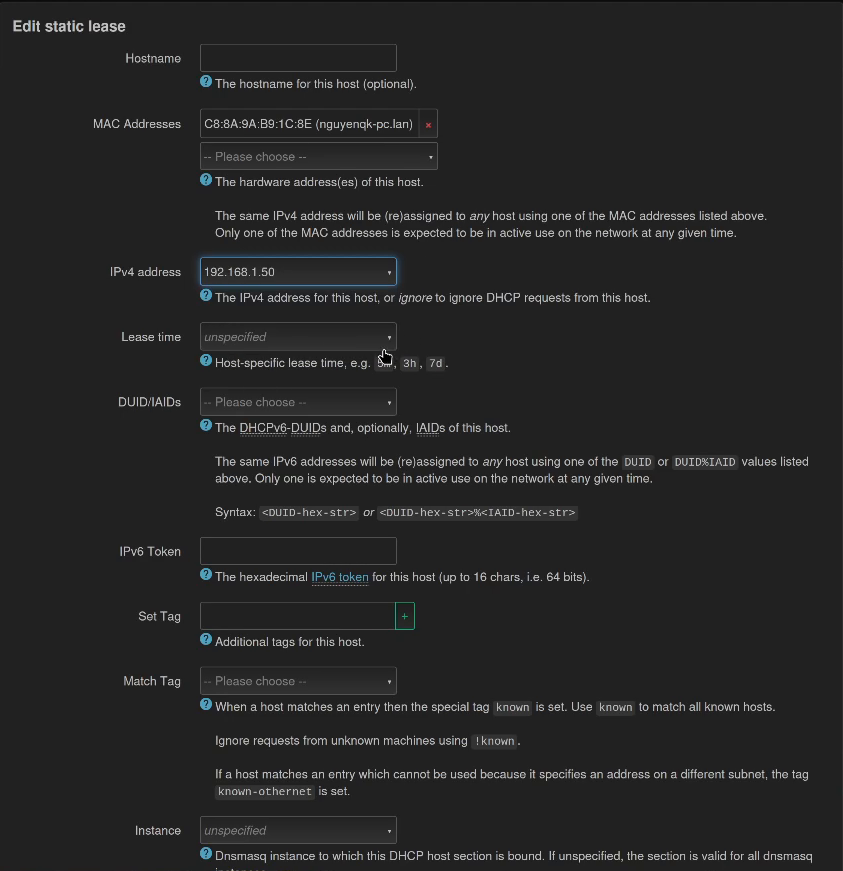
\includegraphics[width=\linewidth]{figures/N09_luci_static_lease.png}
  \caption[Đặt IP tĩnh (Static Lease) cho máy bàn]{Đặt IP tĩnh theo địa chỉ MAC (\emph{Static Lease}) cho máy bàn với địa
  chỉ \texttt{192.168.1.50}.}
  \label{fig:luci-static}
\end{figure}

\begin{table}[htbp]
  \centering\footnotesize
  \caption{Thiết bị nhận địa chỉ từ N09-Router (đọc từ \emph{Active DHCP
  Leases}).}
  \label{tab:dhcp-leases}
  \begin{tabularx}{\linewidth}{@{} L{1.0} L{0.8} L{1.15} L{1.05} @{}}
    \toprule
    \textbf{Hostname} & \textbf{Địa chỉ IPv4} & \textbf{Địa chỉ MAC} &
    \textbf{Thiết bị / kết nối} \\
    \midrule
    \texttt{luckmintpc} & \texttt{192.168.1.216} & \texttt{9C:B1:50:1F:C9:CB} &
      Máy bàn Linux Mint, nối cáp Ethernet vào cổng \ac{lan} \\
    \texttt{nguyenk-pc} & \texttt{192.168.1.145} & \texttt{C8:8A:9A:B9:1C:8E} &
      Laptop Arch Linux, Wi-Fi 5~GHz \\
    \texttt{lzITmeehh} & \texttt{192.168.1.199} & \texttt{24:EB:16:B6:AC:B0} &
      Điện thoại Android, Wi-Fi 5~GHz \\
    \texttt{Redmi-Note-14} & \texttt{192.168.1.115} & \texttt{42:79:95:D5:EC:D2} &
      Điện thoại Redmi Note 14, Wi-Fi 5~GHz \\
    \bottomrule
  \end{tabularx}
\end{table}

\subsection{Minh chứng kết nối thiết bị và kiểm tra chéo}

Sau khi cả bốn thiết bị vào mạng, máy bàn (nguồn đo) lần lượt ping tới từng thiết
bị để kiểm tra khả năng liên lạc qua router (Hình~\ref{fig:ping-shot}). Kết quả
chi tiết ở Bảng~\ref{tab:ping-crosscheck}: hai thiết bị di động phản hồi đủ 4/4
gói, còn thiết bị Android \texttt{lzITmeehh} không phản hồi trong lần đo này dù
vẫn còn trong danh sách thuê DHCP.

\begin{figure}[htbp]
  \centering
  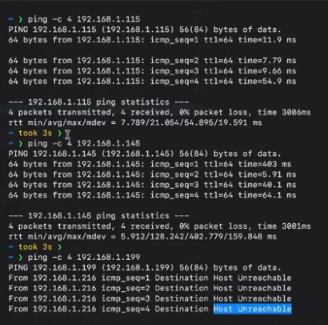
\includegraphics[width=\linewidth]{figures/N09_ping_crosscheck.png}
  \caption[Kiểm tra chéo bằng ping từ máy bàn tới các thiết bị]{Kiểm tra chéo bằng \texttt{ping} từ máy bàn tới các thiết bị trong
  mạng: hai thiết bị phản hồi đủ 4/4 gói, một thiết bị Android trả về
  \emph{Destination Host Unreachable}.}
  \label{fig:ping-shot}
\end{figure}

Ngoài ra, trên máy bàn còn kiểm tra bằng \texttt{nmcli device wifi} để xem danh
sách mạng và kênh đang dùng, và mở trình duyệt để xác nhận truy cập được trang
web khi cổng WAN đã nối. Ảnh chụp màn hình của từng điện thoại (phần cài đặt
Wi-Fi) sẽ được nhóm bổ sung; hiện minh chứng cho các thiết bị này là bảng thuê
DHCP và kết quả ping ở trên.

\subsection{Minh chứng mô hình Ad-hoc (IBSS) hai nút}
\label{subsec:evidence-adhoc}

Trước hết, khả năng hỗ trợ của hệ điều hành được kiểm tra trên máy chủ vật lý
chạy Windows~11. Lệnh \texttt{netsh wlan show drivers} trả về dòng
\emph{Hosted network supported: No} (Hình~\ref{fig:win-hosted}), xác nhận rằng
nền tảng Windows không còn hỗ trợ chế độ ngang hàng, phù hợp với nhận định trong
Mục~\ref{sec:arch}. Vì vậy mạng Ad-hoc được triển khai trên Linux theo quy trình
tại Mục~\ref{sec:adhoc-config}.

\begin{figure}[htbp]
  \centering
  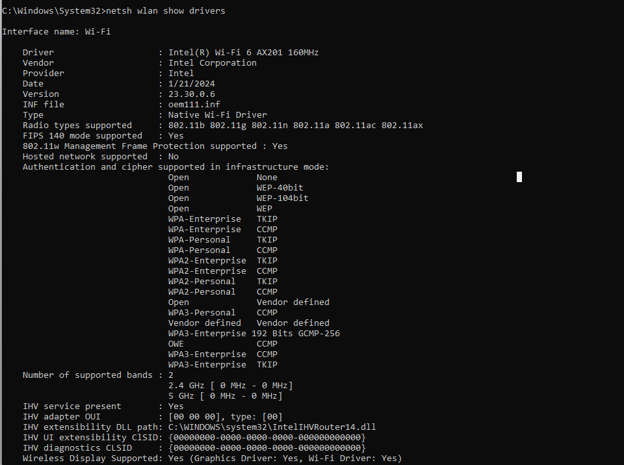
\includegraphics[width=\linewidth]{figures/Picture1.png}
  \caption[Kiểm tra hỗ trợ Ad-hoc trên Windows 11]{Kết quả \texttt{netsh wlan show drivers} trên Windows~11 với dòng
  ``Hosted network supported: No'', cho thấy hệ điều hành không hỗ trợ chế độ
  Ad-hoc.}
  \label{fig:win-hosted}
\end{figure}

Hai card mạng không dây ảo được tạo bằng module \texttt{mac80211\_hwsim} với
tham số \texttt{radios=2}. Kết quả \texttt{iw dev}
(Hình~\ref{fig:hwsim-radios}) xuất hiện hai radio độc lập \texttt{phy\#0} và
\texttt{phy\#1} cùng hai giao diện \texttt{wlan0}, \texttt{wlan1}; giao diện
\texttt{P2P-device} đi kèm \texttt{phy\#1} do trình điều khiển tự tạo để phục vụ
Wi-Fi Direct và không ảnh hưởng đến kết nối Ad-hoc.

\begin{figure}[htbp]
  \centering
  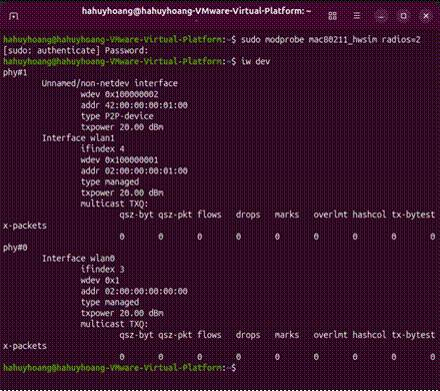
\includegraphics[width=\linewidth]{figures/Picture2.png}
  \caption[Hai radio ảo sau khi nạp \texttt{mac80211\_hwsim}]{Kết quả \texttt{iw dev} sau khi nạp module
  \texttt{mac80211\_hwsim radios=2}: hai radio ảo \texttt{phy\#0} (wlan0) và
  \texttt{phy\#1} (wlan1) được khởi tạo.}
  \label{fig:hwsim-radios}
\end{figure}

Để hai giao diện không dùng chung bảng định tuyến và chuyển gói qua loopback,
mỗi radio được tách vào một network namespace riêng (Hình~\ref{fig:netns}), nhờ
đó mỗi radio hoạt động như một máy tính độc lập.

\begin{figure}[htbp]
  \centering
  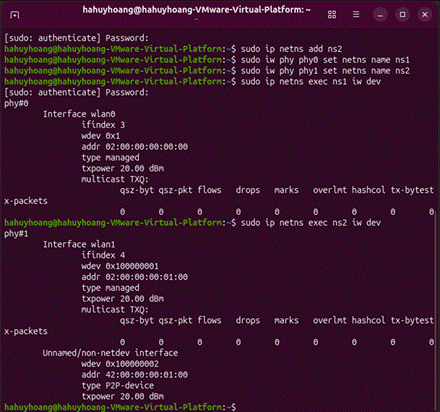
\includegraphics[width=\linewidth]{figures/Picture3.png}
  \caption[Mỗi radio trong một network namespace riêng]{Mỗi radio được gán vào một network namespace riêng: \texttt{ns1} chỉ
  thấy \texttt{phy\#0}, \texttt{ns2} chỉ thấy \texttt{phy\#1}.}
  \label{fig:netns}
\end{figure}

Hai nút được chuyển sang chế độ \ac{ibss}, cùng tham gia một mạng Ad-hoc trên tần
số 2437~MHz (kênh~6) và được gán địa chỉ \texttt{10.0.0.1/24},
\texttt{10.0.0.2/24} (Hình~\ref{fig:adhoc-config}). Lần chạy đầu tiên dùng
\ac{ssid} \texttt{demoAdhoc} như trong ảnh; bản quay minh chứng sau đó dùng
\ac{ssid} \texttt{N09-AdHoc} với cùng kênh và cùng dải địa chỉ, nên hai bộ minh
chứng nhất quán về tham số kỹ thuật.

\begin{figure}[htbp]
  \centering
  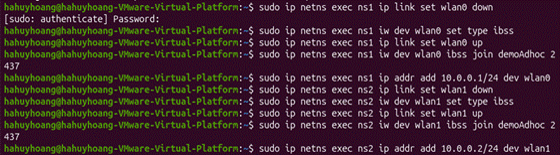
\includegraphics[width=\linewidth]{figures/Picture4.png}
  \caption[Chuỗi lệnh cấu hình chế độ IBSS]{Chuỗi lệnh cấu hình chế độ IBSS cho Node~1 (\texttt{ns1},
  \texttt{wlan0}) và Node~2 (\texttt{ns2}, \texttt{wlan1}).}
  \label{fig:adhoc-config}
\end{figure}

Kết quả kiểm tra ở Hình~\ref{fig:adhoc-check} cho thấy \texttt{wlan0} đang ở
\texttt{type IBSS}, \ac{ssid} của mạng Ad-hoc, kênh~6 (2437~MHz), độ rộng
20~MHz; lệnh \texttt{station dump} ghi nhận nút còn lại với MAC
\texttt{02:00:00:00:01:00} đã ở trạng thái \emph{authorized} và
\emph{associated}, tức hai nút đã nhận ra nhau ở tầng 802.11.

\begin{figure}[htbp]
  \centering
  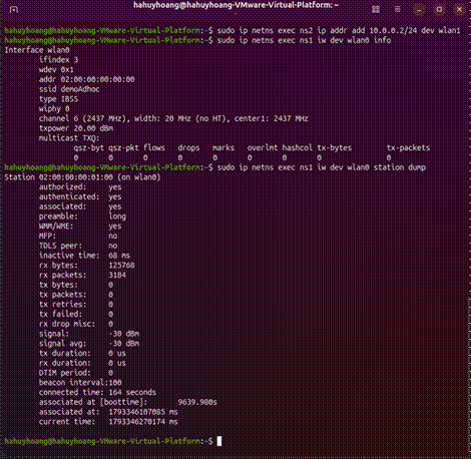
\includegraphics[width=\linewidth]{figures/Picture5.png}
  \caption[Kết quả iw info và station dump]{Kết quả \texttt{iw dev wlan0 info} (type IBSS, kênh~6) và
  \texttt{station dump} (nút lân cận \texttt{02:00:00:00:01:00} đã authenticated
  và associated).}
  \label{fig:adhoc-check}
\end{figure}

Cuối cùng, lệnh ping bốn gói giữa hai nút (Hình~\ref{fig:adhoc-ping}) nhận đủ
4/4 phản hồi, tỉ lệ mất gói 0\,\%, chứng minh mạng Ad-hoc đã hoạt động ở cả tầng
liên kết dữ liệu và tầng mạng.

\begin{figure}[htbp]
  \centering
  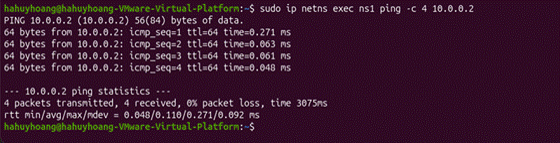
\includegraphics[width=\linewidth]{figures/Picture6.png}
  \caption[Kết quả ping giữa hai nút Ad-hoc]{Kết quả \texttt{ping -c 4 10.0.0.2} từ Node~1 sang Node~2: 4 gói gửi,
  4 gói nhận, mất gói 0\,\%.}
  \label{fig:adhoc-ping}
\end{figure}

\clearpage
\section{Kết quả thử nghiệm và thảo luận}
\label{sec:experiment}

\subsection{Mục tiêu và phạm vi thử nghiệm}
Mục tiêu của phần thử nghiệm là kiểm chứng bằng thực nghiệm hai nội dung lý
thuyết đã trình bày: (i) mô hình hạ tầng cho phép nhiều thiết bị đầu cuối cùng
truy cập tài nguyên qua một \ac{ap} trung tâm, có cấp địa chỉ tập trung và có
bảo mật hiện đại; (ii) mô hình Ad-hoc (\ac{ibss}) cho phép hai thiết bị liên lạc
trực tiếp với nhau mà không cần \ac{ap}. Phần (i) được thực hiện trên router thật
TP-Link Archer C20 v5 chạy OpenWrt với bốn thiết bị đầu cuối; phần (ii) được thực
hiện trên máy ảo Ubuntu vì các thiết bị thật của nhóm đều không còn hỗ trợ
\ac{ibss}.

\subsection{Thiết bị và mô hình thử nghiệm}
Môi trường của hai phần thử nghiệm được tóm tắt trong
Bảng~\ref{tab:moitruong-thunghiem}.

\begin{table}[htbp]
  \centering\footnotesize
  \caption{Môi trường thử nghiệm của hai mô hình.}
  \label{tab:moitruong-thunghiem}
  \begin{tabularx}{\linewidth}{@{} L{0.65} L{1.2} L{1.15} @{}}
    \toprule
    \textbf{Hạng mục} & \textbf{Mô hình hạ tầng} & \textbf{Mô hình Ad-hoc} \\
    \midrule
    Thiết bị trung tâm & TP-Link Archer C20 v5, OpenWrt, tên máy
      \texttt{N09-Router} & Không có \ac{ap} \\
    Giao diện vô tuyến & MT7628 (2,4~GHz, 802.11b/g/n) và MT7610E (5~GHz,
      802.11ac) & Hai card ảo \texttt{phy\#0}, \texttt{phy\#1} do
      \texttt{mac80211\_hwsim} sinh ra \\
    Băng tần, kênh & Kênh~6 (2,4~GHz) và kênh~36 (5~GHz) & Kênh~6 (2437~MHz),
      độ rộng 20~MHz \\
    \ac{ssid} & \texttt{25CLC04-N09} và \texttt{25CLC04-N09-5G} &
      \texttt{N09-AdHoc} \\
    Địa chỉ IP & DHCP \texttt{192.168.1.0/24}, cổng \texttt{192.168.1.1} &
      Tĩnh: \texttt{10.0.0.1/24} và \texttt{10.0.0.2/24} \\
    Bảo mật & WPA2-PSK, mã hóa CCMP (AES) & Mạng mở (không \ac{wep}, không
      WPA2/WPA3) \\
    Thiết bị tham gia & Máy bàn có dây, một laptop và hai điện thoại & Hai
      network namespace trên một máy ảo Ubuntu 22.04 \\
    \bottomrule
  \end{tabularx}
\end{table}

\subsection{Quy trình và kết quả kiểm tra}

\paragraph{Kiểm tra mô hình hạ tầng.} Quy trình gồm: cấu hình router
(Mục~\ref{sec:configuration-guide}), cấp địa chỉ cho thiết bị, kiểm tra liên lạc
với cổng mặc định và giữa các thiết bị, rồi thử các chức năng quản lý. Kết quả
cấp địa chỉ ở Bảng~\ref{tab:dhcp-leases}; kết quả kiểm tra chéo ở
Bảng~\ref{tab:ping-crosscheck}.

\begin{table}[htbp]
  \centering\footnotesize
  \caption{Kết quả ping chéo trong mạng hạ tầng (nguồn: máy bàn
  \texttt{192.168.1.216}).}
  \label{tab:ping-crosscheck}
  \begin{tabularx}{\linewidth}{@{} L{0.85} L{1.0} L{0.75} L{1.4} @{}}
    \toprule
    \textbf{Đích} & \textbf{Thiết bị} & \textbf{Gói nhận} &
    \textbf{RTT min/avg/max/mdev (ms)} \\
    \midrule
    \texttt{192.168.1.115} & Redmi Note 14, Wi-Fi 5~GHz & 4/4 (0\,\%) &
      7,789 / 21,054 / 54,895 / 19,591 \\
    \texttt{192.168.1.145} & Laptop Arch Linux, Wi-Fi 5~GHz & 4/4 (0\,\%) &
      5,912 / 128,242 / 402,779 / 159,848 \\
    \texttt{192.168.1.199} & Điện thoại Android, Wi-Fi 5~GHz & 0/4
      (100\,\%) & Không có: cả bốn gói trả về \emph{Destination Host
      Unreachable} \\
    \bottomrule
  \end{tabularx}
\end{table}

\paragraph{Kiểm tra mô hình Ad-hoc.} Kết quả kiểm tra mạng Ad-hoc hai nút được
tổng hợp ở Bảng~\ref{tab:adhoc-results}.

\begin{table}[htbp]
  \centering\footnotesize
  \caption{Kết quả kiểm tra mạng Ad-hoc hai nút.}
  \label{tab:adhoc-results}
  \begin{tabularx}{\linewidth}{@{} L{0.8} L{0.9} L{1.3} @{}}
    \toprule
    \textbf{Nội dung kiểm tra} & \textbf{Lệnh} & \textbf{Kết quả quan sát} \\
    \midrule
    Giao diện ở chế độ Ad-hoc & \texttt{iw dev wlan0 info} &
      \texttt{type IBSS}, kênh~6 (2437~MHz), độ rộng 20~MHz \\
    Phát hiện nút lân cận & \texttt{station dump} &
      MAC \texttt{02:00:00:00:01:00}, \emph{authorized} và \emph{associated} bằng
      \emph{yes}, cường độ tín hiệu $-30$~dBm, chu kỳ beacon 100~ms \\
    Liên lạc một chiều & \texttt{ping -c 4 10.0.0.2} &
      4 gói gửi, 4 gói nhận, mất gói 0\,\%, RTT cỡ 0,05--0,27~ms \\
    Liên lạc hai chiều & ping từ Node~2 về \texttt{10.0.0.1} &
      Nhận đủ phản hồi, mất gói 0\,\% \\
    \bottomrule
  \end{tabularx}
\end{table}

\subsection{Thảo luận, hạn chế và hướng khắc phục}
\begin{itemize}[leftmargin=*]
  \item \textbf{Mô hình hạ tầng hoạt động đúng lý thuyết.} Router cấp địa chỉ
    DHCP cho bốn thiết bị, hai bộ phát có \ac{bssid} riêng, và các thiết bị liên
    lạc được với nhau qua router. Các chức năng quản lý ở
    Bảng~\ref{tab:chucnang-router} đều cho kết quả quan sát đúng như mong đợi,
    gồm cả trường hợp mạng khách bị chặn truy cập trang quản trị.
  \item \textbf{Độ trễ Wi-Fi cao và dao động mạnh so với mạng có dây.} RTT tới
    hai điện thoại ở mức 21--128~ms trung bình, có gói lên tới 402~ms, trong khi
    mạng có dây thường dưới 1~ms. Nguyên nhân là cơ chế tiết kiệm điện của thiết
    bị di động và việc phải tranh chấp kênh theo \ac{csmaca}; đây cũng là lý do
    một gói đầu tiên thường chậm do phải phân giải ARP.
  \item \textbf{Một thiết bị không phản hồi dù vẫn còn trong danh sách thuê
    DHCP.} Điện thoại \texttt{lzITmeehh} trả về \emph{Destination Host
    Unreachable} cho cả bốn gói trong lần đo. Đây là bài học thực nghiệm quan
    trọng: bản ghi DHCP chỉ chứng minh thiết bị đã từng nhận địa chỉ, không
    chứng minh thiết bị đang trực tuyến; muốn kết luận phải đối chiếu thêm danh
    sách trạm liên kết (\emph{Associated Stations}) hoặc ping lại.
  \item \textbf{Mô hình Ad-hoc bị giới hạn bởi nền tảng.} Cả Windows~11, Android
    và macOS đều không còn hỗ trợ \ac{ibss}, nên thử nghiệm buộc phải chạy trên
    Linux với card ảo. Điều này khẳng định nhận định ở Mục~\ref{sec:arch} rằng
    Ad-hoc gần như đã rời khỏi thiết bị tiêu dùng.
  \item \textbf{Độ trễ trong mô hình Ad-hoc không đại diện cho Wi-Fi thật.}
    \texttt{mac80211\_hwsim} truyền khung bằng phần mềm trong nhân hệ điều hành,
    không có suy hao, khoảng cách hay di chuyển, nên RTT 0,05--0,27~ms chỉ chứng
    minh đường truyền logic hoạt động. Mô phỏng cũng không thể hiện được nhiễu
    hay chuyển vùng.
  \item \textbf{Hướng khắc phục.} Với mô hình hạ tầng: đo thêm thông lượng bằng
    \texttt{iperf3}, đo suy hao theo khoảng cách và thử chuyển vùng giữa hai
    \ac{ap}. Với mô hình Ad-hoc: lặp lại trên hai máy Linux thật có card hỗ trợ
    \ac{ibss} và thử dạng nhiều chặng (MANET) với giao thức định tuyến AODV hoặc
    OLSR.
\end{itemize}

\endgroup
